\documentclass[
	english,
	ruledheaders=section,
	class=report,
	thesis={type=Report}, % Options: Seminararbeit, bachelor, master
	accentcolor=2d,
	marginpar=false,
	BCOR=5mm,
	parskip=half-,
	fontsize=12pt
]{tudapub}

% Note: This template uses biblatex. Please select biber as the bibliography compiler in your editor.

\addTitleBoxLogo*{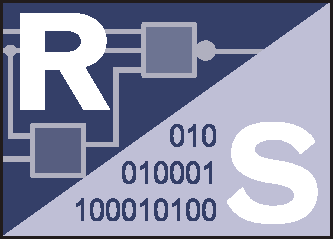
\includegraphics[width=\linewidth,trim=-1.05cm -0.5cm -4.45cm -0.5cm]{bilder/rs_logo}}

% The following block is only needed for pdfTeX on versions before April 2018
\usepackage{iftex}
\ifPDFTeX
\usepackage[utf8]{inputenc}
\fi

%%%%%%%%%%%%%%%%%%%
% Language & Hyphenation
%%%%%%%%%%%%%%%%%%%
\usepackage[english]{babel}
\usepackage[autostyle]{csquotes}% Simplified quotation marks
\usepackage{microtype}

%%%%%%%%%%%%%%%%%%%
% Bibliography
%%%%%%%%%%%%%%%%%%%
\usepackage[sorting=none]{biblatex}
\bibliography{literature}

%%%%%%%%%%%%%%%%%%%
% Tables
%%%%%%%%%%%%%%%%%%%
%\usepackage{array}     % Base package for table configuration, loaded automatically by the following
\usepackage{tabularx}   % Tables that automatically adjust to page width
%\usepackage{longtable} % Multi-page tables
%\usepackage{xltabular} % Multi-page tables with adjustable width
\usepackage{booktabs}   % Improved table layout with horizontal lines

%%%%%%%%%%%%%%%%%%%
% Pseudocode
%%%%%%%%%%%%%%%%%%%
\usepackage{algorithm}
\usepackage{algpseudocode}

%%%%%%%%%%%%%%%%%%%
% Mathematics
%%%%%%%%%%%%%%%%%%%
\usepackage{amsmath}    % Required for pmatrix and math environments
%\usepackage{mathtools} % Extended version of amsmath
%\usepackage{amssymb}   % Extended symbol set
%\usepackage{siunitx}   % Units

%%%%%%%%%%%%%%%%%%%
% RS Template
%%%%%%%%%%%%%%%%%%%
\usepackage{acronym}
\usepackage{listings}

% Packages for AI macros
\usepackage{hyperref}
\usepackage{xparse}
\usepackage{etoolbox}
\usepackage{iflang}
\usepackage{pgfplots}


\lstset{language=C,basicstyle=\small, breaklines=true, showtabs=false, showspaces=false, showstringspaces=false}

\renewcommand{\lstlistingname}{Listing}
\lstset{literate=%
	{Ö}{{\"O}}1
	{Ä}{{\"A}}1
	{Ü}{{\"U}}1
	{ß}{{\ss}}1
	{ü}{{\"u}}1
	{ä}{{\"a}}1
	{ö}{{\"o}}1
}

\begin{document}

\Metadata{
	title=Espresso,
	author=Amey Wankhede
}

\title{Espresso}
\subtitle{Low Level Synthesis - Minitask 1} % optional
\author[Amey Wankhede]{Amey Wankhede} % optional argument is the short name shown in the header

\department{etit}
\institute{
	\IfLanguageName{english}{
		Institute of Computer Engineering
	}{
		Institut für Datentechnik
	}
}
\group{
	\IfLanguageName{english}{
		Computer Systems Group
	}{
		FG Rechnersysteme
	}
}

\reviewer{Prof. Dr.-Ing. Christian Hochberger \and M.Sc. Katharina Schultheis}

\submissiondate{\today}
\examdate{\today}

% AI Macros

% Allow access to macros with @ in their name in order to define the new macro
\makeatletter
\newcommand{\getauthor}{\@author}
\makeatother

\newcommand{\aideclaration}{
	%%%
	% Check which version of the TU template your LaTeX installation uses! The old version uses a section for the affidavit, whereas the new version uses a subsection. Use the appropriate version below and comment out the other one!
	%%%
	\subsection*{Declaration on the Use of Artificial Intelligence}
	%\section*{Declaration on the Use of Artificial Intelligence}

	\begin{sloppypar}%
		I, \getauthor, hereby declare that in this work, artificial intelligence was used, unless otherwise indicated, exclusively for linguistic improvement and formatting assistance. Content generated by artificial intelligence that has not been modified or only slightly adapted is clearly marked and explained in the corresponding section in the appendix.
		\\
	\end{sloppypar}

	\AffidavitSignature
}

\newif\ifainoteseen
\ainoteseenfalse

\newcounter{ainotecounter}
\newcommand{\ainoteentries}{}

\IfLanguageName{english}{%
	\newcommand{\ainote}[2]{%
		\global\ainoteseentrue%
		\stepcounter{ainotecounter}%
		\gappto\ainoteentries{\item \textbf{Model:}~#1 \\ \textbf{Input:}~#2}%
		\hyperlink{ainotes}{\textsuperscript{AI:\theainotecounter}}%
	}
	\robustify\ainote

	\newcommand{\printainoteentries}{%
		\ifainoteseen
		\chapter*{Disclosure of Generated Content}
		\hypertarget{ainotes}{}%
		\begin{enumerate}
			\ainoteentries
		\end{enumerate}
		\fi
	}%
}{%
	\newcommand{\ainote}[2]{%
		\global\ainoteseentrue%
		\stepcounter{ainotecounter}%
		\gappto\ainoteentries{\item \textbf{Model:}~#1 \\ \textbf{Input:}~#2}%
		\hyperlink{ainotes}{\textsuperscript{AI:\theainotecounter}}%
	}
	\robustify\ainote

	\newcommand{\printainoteentries}{%
		\ifainoteseen
		\chapter*{Disclosure of Generated Content}
		\hypertarget{ainotes}{}%
		\begin{enumerate}
			\ainoteentries
		\end{enumerate}
		\fi
	}%
}

% END AI Macros

%	\tuprints{urn=1234,printid=12345}
%	\dedication{For all who use \TeX{}.}

\publishers{}
\maketitle

%\affidavit* % For seminar papers the affidavit is not required and can be commented out.
\aideclaration

\tableofcontents

\chapter{Introduction}

Logic minimization is an essential step in low-level synthesis. The most important parameters for evaluating a logic circuit are its physical area and processing speed. A fundamental unit, such as the universal \ac{NAND} gate, is built using a complementary arrangement of multiple transistors (typically two \ac{NMOS} and two \ac{PMOS}) and can be used to construct any logic circuit. Each logic gate requires a specific amount of time to process a signal and occupies physical space. Consequently, a logic circuit is implemented using various interconnected logic blocks, all of which contribute to the total size and execution time. A logic function can be described as a \ac{SOP}, mapping directly to a \ac{PLA} structure comprising an AND plane and an OR plane. Minimizing the number of literals and product terms reduces the required logic gate count, ultimately yielding a faster and smaller circuit.

Any form of logic minimization is \ac{NP}-hard, meaning no known polynomial-time algorithm exists to find the optimal solution. However, with heuristics, that is, obtaining a solution that works well enough, the problem becomes tractable. That is where the Espresso algorithm comes in.

Espresso was developed by Brayton, Hachtel, McMullen, Rudell and Sangiovanni-Vincentelli at UC Berkeley (1984)\cite{demicheli1994}, and is a standard tool used for logic minimization.
The Espresso algorithm is a heuristic-based logic minimization tool that iteratively optimizes a two-level \ac{SOP} representation. Its objective is to group the fixed mathematical minterms of a function into the most efficient cover possible. It achieves this by simultaneously minimizing the total number of product terms (cubes) to reduce the required number of logic gates, and minimizing the number of literals per term to reduce the transistor count per gate, without altering the underlying boolean logic. 

Internally, Espresso operates on three disjoint sets - the ON set, OFF set, and don't-care set (DC set). Espresso iterates through three phases: expand, which enlarges each cube as far as possible without covering the OFF-set; irredundant, which removes redundant cubes from the cover; and reduce, which shrinks cubes to enable better expansions in the next iteration. This loop repeats until no further reduction in the cost function is achievable.

The Espresso implementation presented in the report includes complement set calculation, a cost function defined as a cover size, and three phases of core Espresso algorithm - Expand, irredundant, and Reduce, which iteratively minimizes cost function. The Espresso implmentation is performed in Java, with logic function equivalency checked using ABC \cite{abc}. Each part's implementation is explained in section \textit{Implementation}.\ainote{Claude Sonnet 4.6}{Improve grammar and LaTeX formatting of the report.}
\chapter{Implementation}

This chapter describes the Java implementation of the Espresso algorithm. It covers the data structures used, the BLIF file parsing framework, the build system, and the implementation of the core algorithmic steps: Complement, Expand, Irredundant, and Reduce. Java was chosen for its speed and Object Oriented abstractions.

\section{Data Structure}
\label{sec:datastructure}

The first thing to decide is the choice of data structure for representing Boolean covers. \ac{PCN} is used as the cube representation throughout the implementation. Each literal within a cube is encoded as a 2-bit integer: \texttt{1} (\texttt{0b01}) represents TRUE, \texttt{2} (\texttt{0b10}) represents FALSE, and \texttt{3} (\texttt{0b11}) represents a \ac{DC} condition. This encoding maps directly to efficient bitwise AND and OR operations, which are used extensively throughout the Espresso sub-parts.

The cover is stored as \texttt{List$<$int[]$>$}, backed by a \texttt{LinkedList}, where each \texttt{int[]} array represents a single cube. The index \texttt{cover[i][j]} holds the PCN state of the $j$-th literal in the $i$-th cube. The number of columns (inputs) is fixed for a given function instance, while the number of rows (cubes) varies as the algorithm inserts and removes cubes during minimization. A \texttt{LinkedList} is used because insertions and deletions are faster compared to fixed arrays, which is useful for frequent cube manipulation required by Expand, Irredundant, and Reduce.

As an example, consider the function $F = abc + a'b + c'$, represented in PCN as:

\[
\begin{pmatrix}
1 & 1 & 1 \\
2 & 1 & 3 \\
3 & 3 & 2
\end{pmatrix}
\]

where rows correspond to cubes and columns correspond to literals $a$, $b$, and $c$ respectively.

Additional supporting data structures include primitive \texttt{int[]} arrays for storing literal ordering and \texttt{ArrayList} for sorting literals by weight heuristics during binate variable selection and, ordering during expansion and reduction.

\section{Parsing Framework}

The input to the tool is a \texttt{.blif} file in \ac{BLIF}. Parsing is handled by the \texttt{Blif} class, which reads the file line by line using a \texttt{BufferedReader}. Each \texttt{.names} directive marks the start of a new function block; the subsequent cube lines are parsed into \ac{PCN} \texttt{Cube} objects via a character-by-character switch: \texttt{0} maps to FALSE (\texttt{0b10}), \texttt{1} maps to TRUE (\texttt{0b01}), and \texttt{-} maps to \ac{DC} (\texttt{0b11}). Only on-set cubes (output column \texttt{1}) are supported. The parser also preserves the file preamble so that the minimized result can be written back to a new \texttt{.blif} file in an \texttt{output/} subdirectory, with the cover replaced by the minimized one.

\section{Build System}

The project is built with \texttt{make}. A suffix rule \texttt{.java.class} compiles each source file via \texttt{javac -g}, and the \texttt{classes} target drives compilation of all nine source files in dependency order. Running \texttt{make} from the \texttt{src/} directory produces the \texttt{.class} files; \texttt{make clean} removes them. The tool is then invoked as \texttt{java Main <file.blif>}.

\section{Espresso Implementation}

The \texttt{Espresso} class is the main class of the minimization algorithm. It is instantiated with the list of \texttt{Function} objects produced by the parser. The constructor first converts the bitset-based \texttt{Cube} representation into the \texttt{List$<$int[]$>$} cover format described in Section~\ref{sec:datastructure}, then instantiates one object each of \texttt{Complement}, \texttt{Expand}, \texttt{Irredundant}, and \texttt{Reduce}, passing \texttt{numInputs} to each.

The algorithm has two phases. In the pre-processing phase, the complement of the initial cover is computed once via recursive Shannon expansion (\texttt{Complement}). The cover is then expanded (\texttt{Expand}), which raises literals to \ac{DC} as far as possible without intersecting the complement, followed by a removal of redundant cubes (\texttt{Irredundant}).

The cost function used throughout is the \textbf{number of cubes} $|F|$; minimization terminates when no iteration reduces this count. The main loop iterates Reduce $\to$ Expand $\to$ Irredundant until the cover size no longer decreases:

\begin{algorithm}
\caption{Espresso main loop}
\begin{algorithmic}[1]
\Repeat
    \State $\text{prevSize} \gets |\text{cover}|$
    \State $\text{cover} \gets \textsc{Reduce}(\text{cover})$
    \State $\text{cover} \gets \textsc{Expand}(\text{cover},\, \text{complement})$
    \State $\text{cover} \gets \textsc{Irredundant}(\text{cover})$
\Until{$|\text{cover}| \geq \text{prevSize}$}
\end{algorithmic}
\end{algorithm}

\noindent The minimized cover is stored as \texttt{minimizedCover} and returned via \texttt{getMinimizedCover()}, after which \texttt{Main} converts it back to \texttt{Cube} objects and writes the result to a \texttt{.blif} file.

\section{Complement}

The \texttt{Complement} class computes $F'$ via recursive Shannon expansion. The result is passed to \texttt{Expand} as the off-set, ensuring no conflict between ON-set and Off-set. The three base cases are: an empty cover returns the universe; a cover containing the universal cube returns empty; a single cube applies De Morgan's theorem directly (each TRUE/FALSE literal becomes its own all-\ac{DC} output cube with that literal flipped). Otherwise, a split variable $x$ is chosen, the positive and negative cofactors are complemented recursively, and the results are merged as $F' = x' \cdot F_{x=1}' + x \cdot F_{x=0}'$.

The splitting order is based on  \textbf{variable ordering heuristic}. Before recursing, \texttt{getOrder} counts how often each variable appears as TRUE vs.\ FALSE across all cubes. Variables that appear in both states (\emph{binate}) are split on first, since they reduce the cover size in both cofactors simultaneously. Within that group, variables are sorted by $\min(\text{trueCount}, \text{falseCount})$ descending, favouring the most balanced split. Unate variables follow. This keeps the recursion tree balanced and avoids deep sub-tree depth.

\section{Expand}

The \texttt{Expand} class raises each literal in each cube to \ac{DC} as far as possible without entering the off-set. For each literal, it is tentatively raised to \ac{DC} and \texttt{checkIntersect} verifies the result against every cube in the complement cover: two cubes intersect if and only if their PCN values have a non-zero bitwise AND in every column. If any complement cube intersects, the literal is restored.

The \textbf{weight heuristic} in \texttt{getOrder} orders cubes by ascending dot product of a row vector (the cube's PCN bits) and a column vector (the per-literal TRUE/FALSE occurrence counts across the whole cover). Cubes with a low dot product share few literals with other cubes and are therefore expanded first, they are less likely to block each other's expansion.

\section{Irredundant}

The \texttt{Irredundant} class drops cubes that contribute no unique minterms. For each cube $c$, the cover $F \setminus \{c\}$ is formed and its complement $(F \setminus \{c\})'$ is computed. Cube $c$ is redundant if and only if $c \cap (F \setminus \{c\})' = \emptyset$ - meaning every minterm of $c$ is already covered by the rest. The intersection check reuses the same bitwise test as Expand. Redundant cubes are removed in place.

\section{Reduce}

The \texttt{Reduce} class shrinks each cube to its smallest cover that still holds at least one minterm unique to it, preparing for a different Expand pass. For cube $c_i$, the \emph{supercube} is computed as the bitwise OR of all cubes in $(F \setminus \{c_i\})'$, i.e.\ the region not already covered by the other cubes. The reduced cube is then $c_i \cap \text{supercube}$, computed with a bitwise AND. This guarantees $c_i$ captures minterms that no other cube covers.

The weight heuristic mirrors Expand but sorts in \emph{descending} order, so the most-shared cubes (highest dot product) are reduced first since they have more overlap with others and can be shrunk the most aggressively.\ainote{Claude Sonnet 4.6}{Improve LaTeX formatting and grammar of the Implementation chapter.}


\include{problems}
\chapter{Evaluation}

The implementation was tested on all 20 \ac{BLIF} benchmark files (0--19). Table~\ref{tab:results} compares the initial cube count, the reference minimized count, and the result produced by this implementation. File~11 ($^*$) ran to completion but achieved no reduction (1027 $\to$ 1027), with \texttt{Expand} taking $\approx$45\,s and \texttt{Irredundant} $\approx$10\,min.

\begin{table}[h]
\centering
\begin{tabular}{@{}rrrr@{}}
\toprule
File & Initial & Reference & This work \\
\midrule
0  & 4   & 3   & \textbf{2}   \\
1  & 4   & 1   & 1   \\
2  & 12  & 4   & 4   \\
3  & 8   & 5   & 5   \\
4  & 14  & 7   & 7   \\
5  & 15  & 8   & 8   \\
6  & 28  & 15  & 15  \\
7  & 34  & 17  & 17  \\
8  & 69  & 29  & 29  \\
9  & 64  & 25  & 26  \\
10 & 290 & 182 & 186 \\
11 & 1027 & 771 & 1027$^*$ \\
12 & 156 & 87  & 87  \\
13 & 307 & 117 & 132 \\
14 & 240 & 10  & 10  \\
15 & 481 & 218 & 218 \\
16 & 420 & 86  & 148 \\
17 & 32  & 1   & 1   \\
18 & 46  & 46  & 46  \\
19 & 92  & 20  & 20  \\
\bottomrule
\end{tabular}
\caption{Cube counts before and after minimization.\ainote{Claude Sonnet 4.6}{Format experimental results into a LaTeX table.}}
\label{tab:results}
\end{table}

15 out of 20 tested files match or improve on the reference. File~0 produces a smaller cover than the reference (2 vs.\ 3), indicating the algorithm found a valid alternative minimization. Files~9, 10, 13, and 16 are slightly above the reference, suggesting the Reduce--Expand--Irredundant loop converged to a local minimum rather than the global optimum, which is expected behaviour for the heuristic Espresso algorithm. File~11 produced no reduction at all despite completing.

\section{Functional Equivalence}

Correctness of the minimized outputs was verified using the \texttt{cec} (combinational equivalence checking) command in the ABC logic synthesis tool. The minimized cover was checked against the original for a representative selection of files:

\begin{table}[h]
\centering
\begin{tabular}{@{}lll@{}}
\toprule
File & Result & Time \\
\midrule
1.blif  & Equivalent (structural hashing) & 0.00\,s \\
10.blif & Equivalent                      & 0.02\,s \\
13.blif & Equivalent                      & 0.03\,s \\
18.blif & Equivalent (structural hashing) & 0.00\,s \\
\bottomrule
\end{tabular}
\caption{ABC \texttt{cec} equivalence check results.\ainote{Claude Sonnet 4.6}{Format ABC CEC results into a LaTeX table.}}
\label{tab:cec}
\end{table}

All checked outputs are functionally equivalent to their inputs, confirming that the minimization preserves the Boolean function. This includes file~13, where the cube count is above the reference, verifying that the result is still correct despite being suboptimal.


% Required to avoid problems with figure captions generating two entries, as the macros would be parsed again within the \listoffigures section.
\renewcommand{\ainote}[2]{}

\IfLanguageName{english}{%
	\chapter*{List of Abbreviations}%
}{%
	\chapter*{List of Abbreviations}
}
\begin{acronym}
	\acro{SOP}{Sum of Products}
	\acro{NAND}{Not AND}
	\acro{PLA}{Porgrammable Logic Array}
	\acro{NP}{Non polynomial}
	\acro{NMOS}{N-type Metal-Oxide-Semiconductor}
	\acro{PMOS}{P-type Metal-Oxide-Semiconductor}
	\acro{PCN}{Positional Cube Notation}
	\acro{DC}{Don't care}
	\acro{BLIF}{Berkeley Logic Interchange Format}
\end{acronym}

\nocite{*}
\printbibliography

\printainoteentries

\end{document}
